% Created 2018-06-25 Mo 13:07
% Intended LaTeX compiler: pdflatex
\documentclass[journal abbreviation, manuscript]{copernicus}
\usepackage[utf8]{inputenc}
\usepackage[T1]{fontenc}
\usepackage{graphicx}
\usepackage{grffile}
\usepackage{longtable}
\usepackage{wrapfig}
\usepackage{rotating}
\usepackage[normalem]{ulem}
\usepackage{amsmath}
\usepackage{textcomp}
\usepackage{units}
\usepackage{amssymb}
\usepackage{natbib}
\usepackage{capt-of}
\usepackage{hyperref}
\author{simon}
\date{\today}
\title{}
\hypersetup{
 pdfauthor={Simon Pfreundschuh},
 pdftitle={},
 pdfkeywords={},
 pdfsubject={},
 pdfcreator={Emacs 24.5.1}, 
 pdflang={English}}
\begin{document}

\setlength{\parindent}{0cm}

\section*{Interactive comment on ``A neural network approach to estimate a posteriori distributions of Bayesian retrieval problems'' by Simon Pfreundschuh et al.}

\section{Comments from first referee}

\subsection*{Referee comment:}

P. 15: in the comparisons between QRNN and the BMCI, as the training data or a-prior
get smaller, the BMCI uncertainties need to be increased beyond the sensor noise to
account for a sparse a-priori.  If that was not done, it likely explains the divergence in
the performance for smaller training sets.  That said, finding the uncertainty due to a
sparse a-priori is not at all trivial so it might still be an advantage for the QRNN but
perhaps slightly different than presented. A bit more explanation by the author on this
topic would help the paper. The conclusion mentions this as well.

\subsection*{Author response:}

This is a very valid point that has indeed not been considered in the presented
calculations. However, in particular since there is no formal way of doing this,
it seems that finding suitable ways of handling scarce databases with BMCI would
merit a study of its own. Applying just any ad-hoc solution to increase the
measurement uncertainty is unlikely to do the BMCI method justice, so the authors
judge it to be out of the scope of the study to investigate this further.

To address this in the manuscript, the following paragraph has been added:

\vspace{1em}

\textit{
A possible approach to handling scarce retrieval databases with BMCI is to
artificially increase the assumed measurement uncertainty. This has not been
performed for the BMCI results presented here and may improve the performance of
the method. The difficulty with this approach is that the method formulation
is based on the assumption of a sufficiently large database and thus can,
at least formally, not handle scarce training data. Finding a suitable way to
increase the measurement uncertainty would thus require either additional
methodological development or invention of an heuristic approach, both of which
are outside the scope of this study.}

\subsection*{Referee comment}

P. 12, line 12:  Maybe I missed it but I don’t think Rectilinear Linear Unit was ever
defined in the paper.

\subsection*{Author response}

The ReLU activation function is now introduced as Rectified Linear Unit the
first time the acronym is used in the text.

\subsection*{Referee comment}
I am quite certain that neither “Gaussianity” (p.3, line 2) nor “overproportionally” (p. 12,
line 20) are real words.

\subsection*{Author response}

The word \emph{Gaussianity} has been replaced. The sentence now reads:

\vspace{1em}
\textit{
Nonetheless, even neglecting the validity of the assumptions of Gaussian
a priori and measurement errors as well as linearity of the forward
model, the method is unsuitable for retrievals that involve complex
radiative processes.
}
\vspace{1em}

Similarly, \emph{overproportionally} (which correctly should have been
overpropotionately) has been replaced by \emph{excessively}.

\subsection*{Referee comment}

p. 4, line 15: There is an extra “from” in front of “directly”

\subsection*{Author comment}

The word \emph{from} has been removed.

\section{Comments from second referee}

\subsection{General comments}

\subsection*{Referee comment:}

1) While I think that examining bias histograms of retrieval variables is a useful way
of  evaluating  retrieval quality,  it  would be  useful to  provide readers  a picture  of the
behavior of the original histograms.  To that end, I think that, in addition to figure 8, a
1-D histogram (pressure on the vertical axis) of predicted cloud top pressures should
be shown (including each of the 3 approaches).

\subsection*{Author response:}

The following figure has been added to the manuscript:

  \begin{center}
  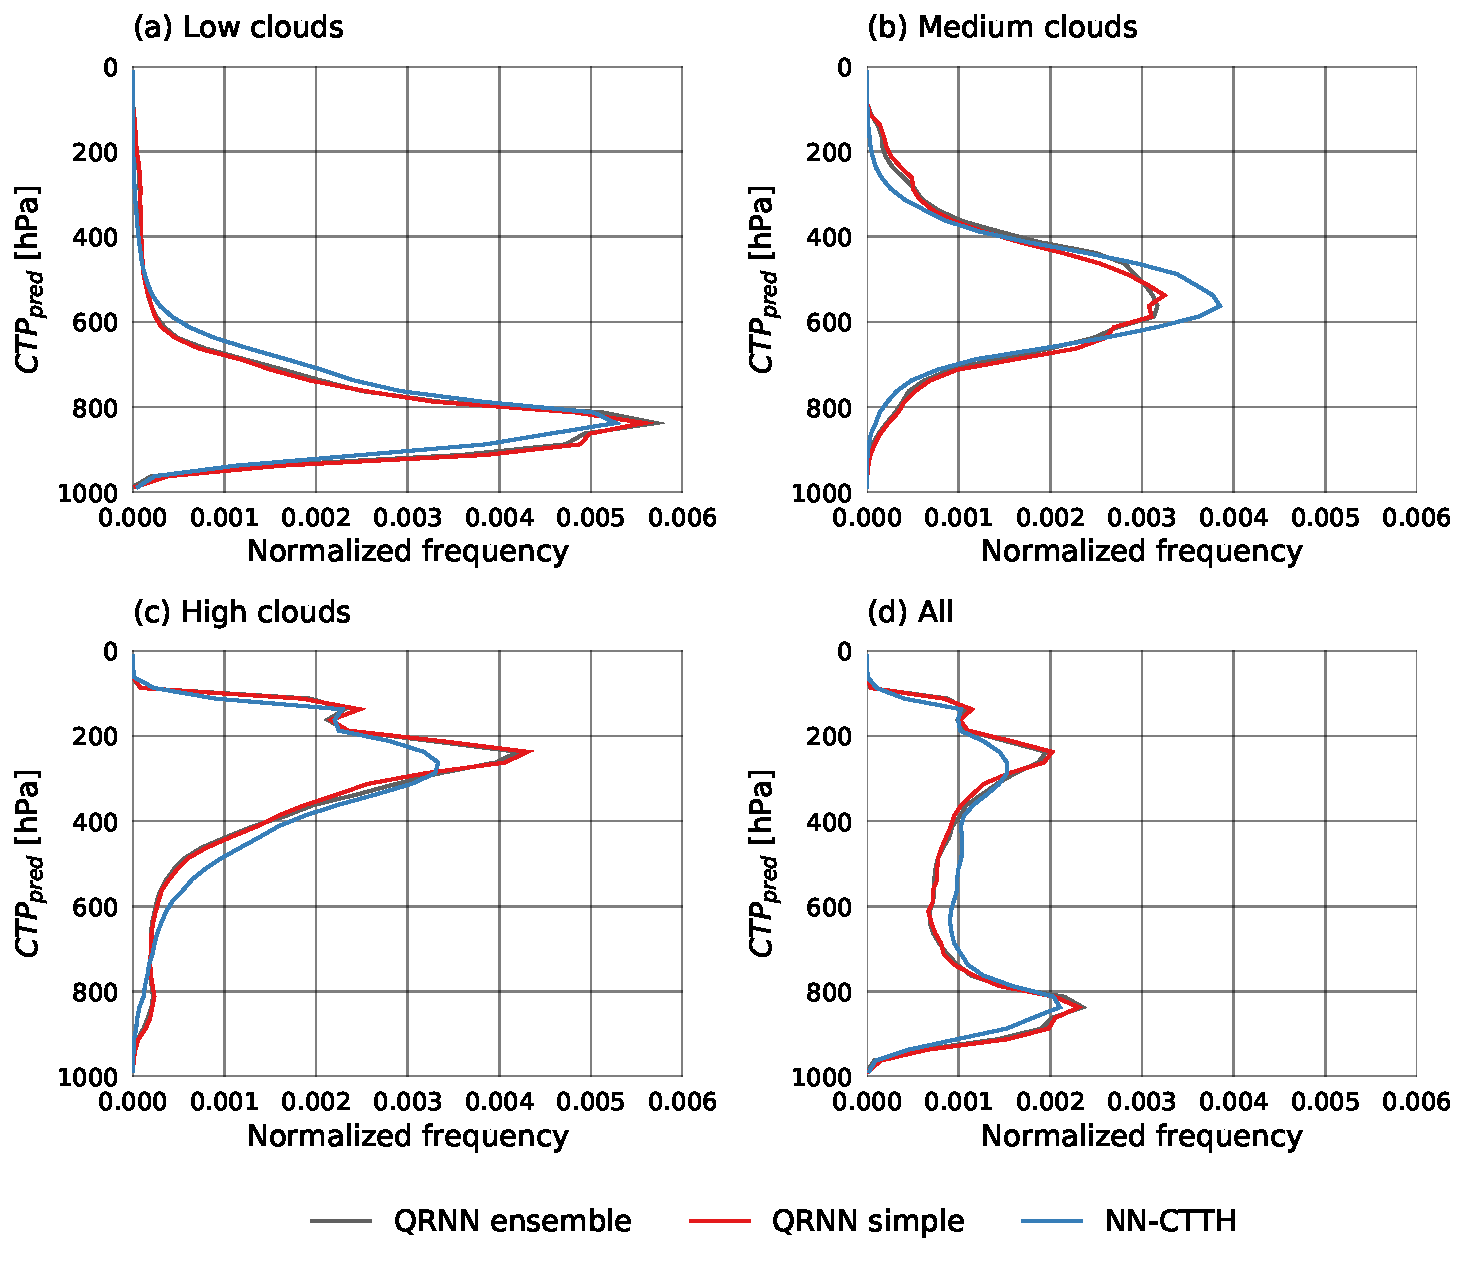
\includegraphics[width = 0.8\linewidth]{../plots/fig09}
  \end{center}


\vspace{1em}

Furthermore, the accompanying discussion of the single value retrieval results
has been extended and now reads:

\vspace{1em}

\begin{em}
Most data analysis will likely require a single predicted value for the cloud top
pressure. To derive a point value from the QRNN prediction, the median of the
estimated a posteriori distribution is used.

The distributions of the resulting median pressure values 
on the \textit{testing during development} data set are displayed in
Figure~8 together with the retrieved pressure
values from the NN-CTTH algorithm. The distributions are displayed
separately for low, medium and high clouds (as classified by the CALIOP
feature classification flag) as well as for the complete data set. From these
results it can be seen that the values predicted by the QRNN have stronger peaks
low in the atmosphere for low clouds and high in the atmosphere for
high clouds. For medium clouds the peak is more spread out and has heavier
tails low and high in the atmosphere than the values retrieved by the NN-CTTH
algorithm.

Figure~9 displays the error distributions of the predicted
CTP values on the \textit{testing during development} data set, again seperated by
cloud type as well as the complete data set. Both the simple QRNN and the ensemble
of QRNNs perform slightly better than the NN-CTTH algorithm for low and high clouds.
For medium clouds, no significant difference in the performance of the methods can
be observed. The ensemble of QRNNs seems to slightly improve upon the prediction
accuracy of a single QRNN but the difference is likely negligible. Compared to
the QRNN results, the CTP predicted by NN-CTTH is biased low for low clouds and
biased high for high clouds.

Even though both the QRNN and the NN-CTTH retrieval use the same input and
training data, the predictions from both retrievals differ considerably. Using
the Bayesian framework, this can likely be explained by the fact that the two
retrievals estimate different statistics of the a posteriori distribution. The
NN-CTTH algorithm has been trained using a squared error loss function which
will lead the algorithm to predict the mean of the a posteriori distribution.
The QRNN retrieval, on the other hand, predicts the median of the a posteriori
distribution. Since the median minimizes the expected absolute error, it is
expected that the CTP values predicted by the QRNN yield overall smaller errors.
\end{em}

\subsection*{Referee comment:}

2) I understand the usage of the CDF’s in figure 3 to demonstrate the statistical value of
the retrievals, but again, I think you need to directly show at least an example of a 1-D
histogram of the retrieved variable. It gives readers a more direct sense of the variable
being retrieved and provides context.

\subsection*{Author response:}

The following figure and accompanying text have been added to the manuscript:

    \begin{center}
    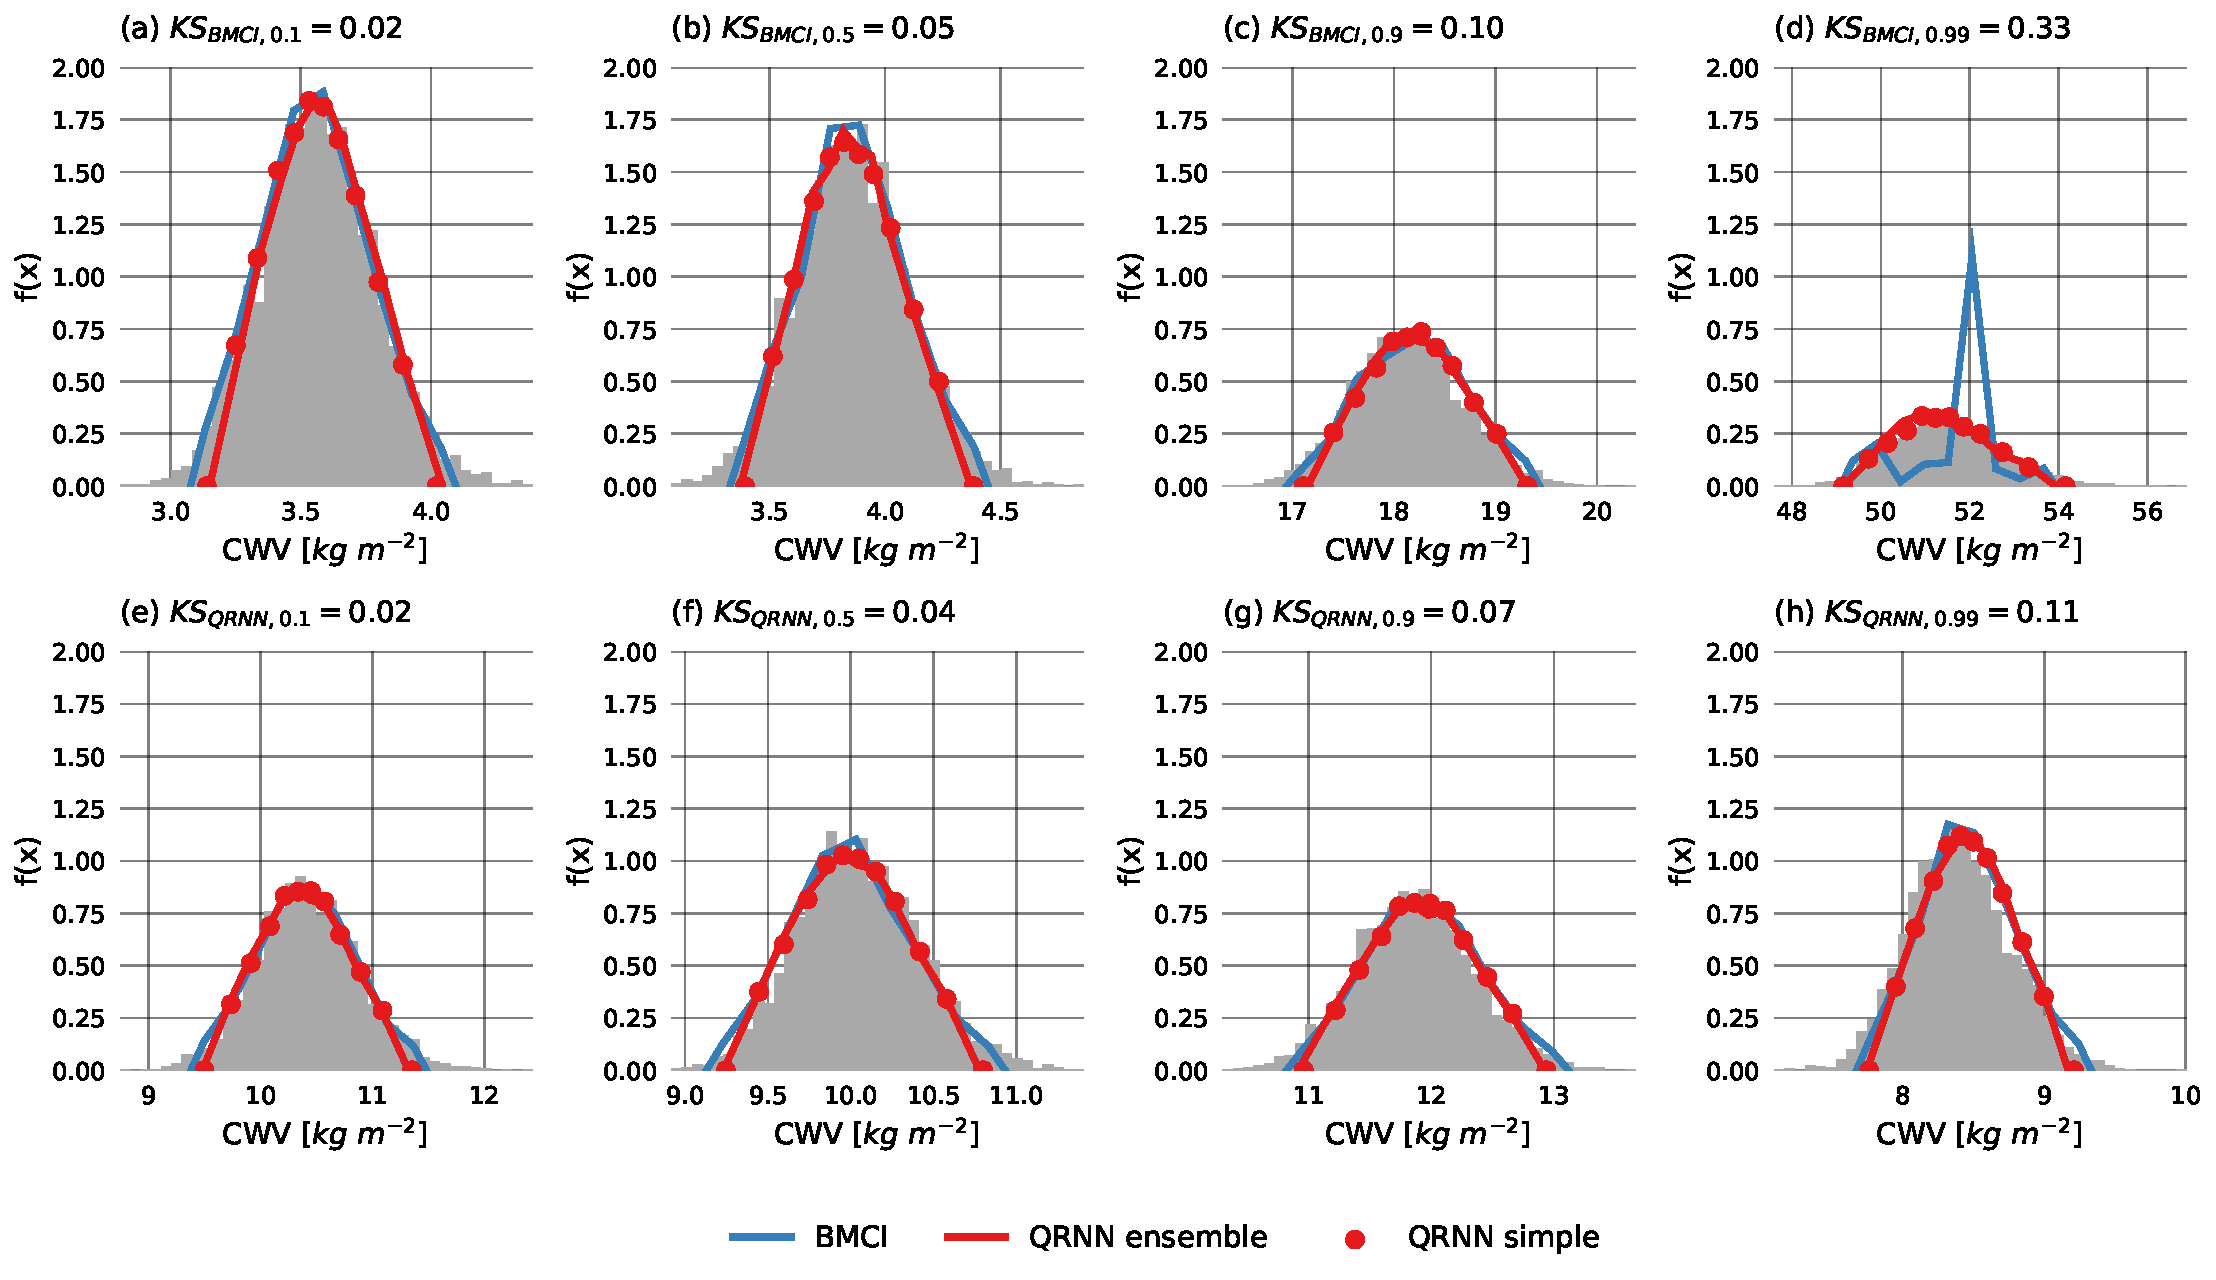
\includegraphics[width = 1.0\linewidth]{../plots/fig04}
    \end{center}

\begin{em}
  Another way of displaying the estimated a posteriori distribution is by means
  of its probability density function (PDF), which is defined as the derivative
  of its CDF. For the QRNN, the PDF is approximated by simply deriving
  the piece-wise linear approximation to the CDF and setting the boundary values
  to zero. For BMCI, the a posteriori PDF can be approximated using a histogram
  of the CWV values in the database weighted by the corresponding weights
  $w_i(\mathbf{y})$. The PDFs for the cases corresponding to the CDFs shown in
  Figure~3 are shown in Figure~4.
\end{em}

\subsection{Specific comments}

\subsection*{Referee comment:}

1. Page 2, Line 31: Abbreviations of MAP and 1DVAR are undefined.

\subsection*{Author response:}

The abbreviation MAP has been removed since it neither commonly used nor
and accurate designation of the method. The following explanation of the
name 1DVAR has been added:

\vspace{0.5em}
\textit{(also 1DVAR, for one-dimensional variational retrieval)}

\subsection*{Referee comment:}
2. Page 4, Line 15: The sentence at the beginning of section 2.2 would almost be better
suited as a conclusory sentence at the end of section 2.1. As a matter of formatting, I
think it’s best to avoid a section being a single sentence long.

\subsection*{Author response:}

The sentence at the beginning of the paragraph was meant as an introduction to the
subsection on Bayesian methods. In the hope that this aids both the formatting as
well as the readability this introductory part has been changed to:


\vspace{1em}
\textit{
Bayesian retrieval methods are methods that use the expression for the a
posteriori distribution in Eq. (1) to compute a solution to the
retrieval problem. Since the a posteriori distribution can generally not be
computed or sampled directly, these methods approximate the posterior
distribution to varying degrees of accuracy.}

\subsection*{Referee comment:}

3. Page 9, Line 5: Can you provide an explanation for this restriction of latitudes in the
dataset?
\subsection*{Author response:}

We restricted the data set to the mid-latitudes regime in the hope that this
would make the temperature and water vapor profiles more simple to represent
using multivariate (Log-)Gaussian distributions. However, since this choice
was rather arbitrary and not considered essential for the following analysis,
we decided to not explicitly state this in the manuscript.

\subsection*{Referee comment:}

4.  Page 10, Line 8:  The formatting of this citation for Typhon seems like it might be
incomplete or incorrect for the type of source being cited.

\subsection*{Author response:}

The AMT guidelines for manuscript preparation do not contain guidelines on how to
cite software. The reference format used here seemed most plausible to us and
is also the one recommended by the typhon developers. Nonetheless, if the referee
has suggestions to improve the citation format, we would be more than happy to
consider them.

\subsection*{Referee comment:}

5. Page 10, Line 19: I don’t follow the statement, “not smaller than and larger than 100,
respectively”.  I read that as a logical statement that can’t be possible because of the
usage of “and.” Do you perhaps mean “or?”

\subsection*{Author response:}

The statement is indeed unnecessarily complicated and probably logically incorrect. It has been
rewritten and now reads:

\vspace{0.5em}
\textit{
  The retrieval is accepted only if the scale reduction factor is smaller than 1.1
  and the effective sample size larger than 100.
}

\subsection*{Referee comment:}

6.  Page 10, Line 24: Missing word.  Need to insert as into, ”It is also released as part
of the typhon package.

\subsection*{Author response:}

The missing word has been inserted.

\subsection*{Referee comment}

7.  Page 15, Line 30:  NN-CTTH is an undefined abbreviation.  Because of the similarity
to the abbreviation for cloud top height (CTH) I almost didn’t notice that I didn’t
understand the name of the algorithm until later in the paper.

\subsection*{Author response}

We agree with the referee that the introduction of NN-CTTH as name of the retrieval
algorithm was not very clear. The relevant phrase has been reformulated and now reads:

\vspace{0.5em}
\textit{
  This experiment is based on the work by \citet{hakansson} who
developed the NN-CTTH algorithm, a neural network based retrieval of cloud top
pressure.}



\subsection*{Referee comment}

8. Page 17, Line 2: This feels like an incomplete sentence. Perhaps if you reorder it a
bit it will make more sense.  For example:  “The NN-CTTH algorithm and the QRNN
are trained using the exact same data set. This training set consists
...
”


9.  Page 17, Line 7:  I also recommend reorganizing this sentence:  “In Håkansson et
al.  (2018) neural networks are trained using different combinations of input features
(e.g., [example from paper goes here]) in order to evaluate network performance with
different inputs.”


10. Page 17, Line 12-14: I don’t follow along with this paragraph. Is the “testing under
development” dataset the same as the AVHRR version?  Could you clarify this para-
graph some?  Right now it seems that the confusion stems from the discussion of two
different datasets within the space of only three sentences – making I difficult to clarify
the difference between them. Is the first sentence referring to the first paragraph?

\subsection*{Author response}

In the hope of making it easier to read and understand, the subsection has been
revised and now reads:

\vspace{0.5em}

\begin{em}
The QRNN uses the same data for training as the reference NN-CTTH algorithm. The
data set consists of MODIS Level 1B data \citep{myd021km, myd03} collocated with
cloud properties obtained from CALIOP \citep{calipso}. The top layer
  pressure variable from the CALIOP data is used as retrieval target. The data
was taken from all orbits from 24 days (the 1st and 14th of every month) from
the year 2010. In \citet{hakansson} multiple neural networks are trained using
varying combinations of input features derived from different MODIS channels and
ancillary NWP data in order to compare retrieval performance for different
inputs. Of the different neural network configurations presented in
\citet{hakansson}, the version denoted by NN-AVHRR is used for comparison
against the QRNN. This version uses only the $11 \unit{\mu m}$ and $12\unit{\mu
  m}$ channels from MODIS. In addition to single pixel input, the input features
comprise structural information in the form of various statistics computed on a
$5 \times 5$ neighborhood around the center pixel. The ancillary numerical weather
prediction data provided to the network consists of surface pressure and
temperature, temperatures at five pressure levels, as well as column integrated
water vapor. These are also the input features that are used for the training of
the QRNN. The training data used for the QRNN are the training and
during-training validation set from \citet{hakansson}. The comparison to
the NN-AVHRR version of the NN-CTTH algorithm uses the data set for
testing under development from \cite{hakansson}.
\end{em}



\subsection*{Referee comment}

11. Page 17, Line 16-17: This sentence is a little confusing to read.

\subsection*{Author response}

In the hope of making the sentence less confusing it has been rewritten
and now reads:

\vspace{0.5em}
\textit{
The training progress, based on which the
learning rate is reduced or training aborted, is monitored using the
during-training validation data set from \cite{hakansson}.
}

\subsection*{Referee comment}

12.  Page 18, Line 6-7:  Could you expand on how the performance for low and high
clouds differs here?  Because you’re discussing in terms of low and high clouds and
cloud top pressure it’s useful to highlight that a negative CTPpred-CTPref means that
the cloud is higher than the reference.  Basically, for the NN-CTTH low clouds have a
high-bias and high clouds have a low-bias. It’s useful to say that explicitly.

\subsection*{Author response}

This has been addressed as part of the general comment 1.).

\subsection*{Referee comment}

13.  Page 23, Line 20:  For the sake of clarity for a more general audience can you
provide an example of a vector-valued retrieval quantity.

\subsection*{Author response}

The sentence has been rewritten and now includes an example of a
vector-valued retrieval quantity:

\vspace{0.5em}
\textit{
Another aspect of the application of QRNNs to remote sensing retrievals that
remains to be investigated is how they can be used to retrieve vector-valued
retrieval quantities, such as for example concentration profiles of atmospheric gases or
particles.
}

\bibliographystyle{copernicus}
\bibliography{literature}

\end{document}
